[84~r\textsuperscript{o}]  Cardo hujus rei in hoc versatur ut magnam radiorum parallelorum copiam per vitrum in quod incidunt ita refringi faciamus, ut postea ad unum idemque; punctum tendant. Sed punctum hoc aut mathematice aut mechanice considerari potest. Et quamvis certum sit, figuras circulares non habere potentiam illam aut proprietatem,  (ut quidem Ellipticae aut hyperbolicae, ac infinitae aliae  magis compositae) parallelos radios ita refringendi, ut  postea ad unum punctum Mathematicum\protect\index{Sachverzeichnis}{punctum!mathematicum} tendant, nihilominus tamen, magnam eorum copiam ita versus eundem  locum inflectere possunt, ut spatium illud in quo omnes  conveniunt, pro mechanico puncto\protect\index{Sachverzeichnis}{punctum!mechanicum} tantum sit habendum. Punctum autem mechanicum\protect\index{Sachverzeichnis}{punctum!mechanicum} appello, quod in mechanicis  aut divisibile non est, aut cujus partes hic non sunt  consideratu dignae.\pend
  % \begin{wrapfigure}{l}{0.4\textwidth}                    
%    \begin{center}  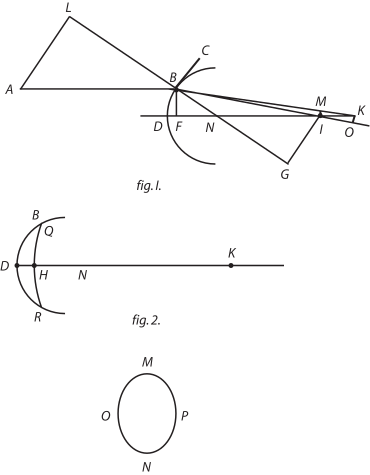
\includegraphics[width=0.7\textwidth]{images/37_02_084r123.pdf}
%    \\\hspace{-24mm}\textit{[Fig. 3]}
%    \end{center}
 
                        %\caption{Bildbeschreibung}
                        %\end{wrapfigure}
                        %@ @ @ Dies ist eine Abstandszeile - fuer den Fall, dass mehrere figures hintereinander kommen, ohne dass dazwischen laengerer Text steht. Dies kann zu einer Fahlermeldung fuehren. @ @ @ \\
                   % \begin{wrapfigure}{l}{0.4\textwidth}                    
                %\includegraphics[width=0.4\textwidth]{../images/Zu+Johann+Hudde%2C+Specilla+circularia/LH037%2C02_084r/files/100087.png}
                        %\caption{Bildbeschreibung}
                        %\end{wrapfigure}
                        %@ @ @ Dies ist eine Abstandszeile - fuer den Fall, dass mehrere figures hintereinander kommen, ohne dass dazwischen laengerer Text steht. Dies kann zu einer Fahlermeldung fuehren. @ @ @ \\
                     % \begin{wrapfigure}{l}{0.4\textwidth}                    
                %\includegraphics[width=0.4\textwidth]{../images/Zu+Johann+Hudde%2C+Specilla+circularia/LH037%2C02_084r/files/100089.png}
                        %\caption{Bildbeschreibung}
                        %\end{wrapfigure}
                        %@ @ @ Dies ist eine Abstandszeile - fuer den Fall, dass mehrere figures hintereinander kommen, ohne dass dazwischen laengerer Text steht. Dies kann zu einer Fahlermeldung fuehren. @ @ @ \\
                     